% Density revision 2026-10-04: answers below questions; compact related content.
% ৪.x HTML-এ লেখা বিন্যাস
\section{HTML-এ লেখা বিন্যাস (Text Formatting)}

% Composition pass 2026-10-04
একটি বিজ্ঞপ্তিতে শিরোনাম, অনুচ্ছেদ ও গুরুত্বপূর্ণ শব্দ একইভাবে দেখালে পড়া কঠিন হয়।

\chFourMotivation{লেখার স্তর ও গুরুত্ব বোঝানো $\rightarrow$ বিন্যাসের ট্যাগ $\rightarrow$ শিরোনাম, অনুচ্ছেদ ও জোর দেওয়ার অংশ চিহ্নিত করা $\rightarrow$ পাঠযোগ্য কলেজ নোটিশ।}


\begin{learningbox}
এই অংশ শেষে শিক্ষার্থী পারবে:
\begin{itemize}
\item HTML-এ লেখা বিন্যাস কী তা ব্যাখ্যা করতে।
\item শিরোনাম, অনুচ্ছেদ, লাইন বিরতি ও অনুভূমিক বিভাজক ট্যাগ ব্যবহার করতে।
\item মোটা অক্ষরের, বাঁকা অক্ষরের, নিচে রেখাযুক্ত, যোগ করা, বাদ দেওয়া, নিচের সূচক, উপরের সূচক ও উৎসের বিন্যাস অক্ষুণ্ণ রাখা লেখা ট্যাগ লিখতে।
\item \texttt{<font>} ট্যাগের \texttt{size}, \texttt{color}, \texttt{face} অ্যাট্রিবিউট ব্যাখ্যা করতে।
\item রং, পটভূমির রং ও লেখা সাজানোর অবস্থানের মৌলিক HTML/CSS রীতি বুঝতে।
\item HSC-এর ব্যবহারিক অনুশীলনের কোডে লেখা বিন্যাস ট্যাগ প্রয়োগ করতে।
\item \texttt{<marquee>} ট্যাগের মৌলিক \texttt{direction} অ্যাট্রিবিউট চিনতে।
\end{itemize}
\end{learningbox}



\subsection{লেখা বিন্যাস কী?}

\begin{definitionbox}{লেখা বিন্যাস (Text Formatting)}
HTML ট্যাগ দিয়ে লেখার ধরন, গুরুত্ব ও উপস্থাপন নির্ধারণের প্রক্রিয়াকে লেখা বিন্যাস বলে। অক্ষরের আকার, রং ও অবস্থান নিয়ন্ত্রণে CSS-ও ব্যবহৃত হয়।
\end{definitionbox}

বিন্যাসের ট্যাগ দিয়ে লেখাকে মোটা বা বাঁকা অক্ষরে এবং নিচে রেখাসহ দেখানো যায়। ছোট-বড় অক্ষর, নিচের ও উপরের সূচক, যোগ করা বা বাদ দেওয়া লেখা এবং উৎসের ফাঁক ও লাইনবিরতিও প্রকাশ করা যায়। সঠিক বিন্যাসে পাঠক লেখার স্তর ও গুরুত্বপূর্ণ অংশ সহজে বুঝতে পারেন।



\subsection{শিরোনামের ট্যাগ: \texttt{<h1>} থেকে \texttt{<h6>}}

\begin{definitionbox}{শিরোনামের ট্যাগ (Heading Tag)}
ওয়েবপেজের বিষয়বস্তুর শিরোনাম ও তার স্তর প্রকাশের জন্য ব্যবহৃত HTML ট্যাগকে শিরোনামের ট্যাগ বলে।
\end{definitionbox}

HTML-এ ছয় স্তরের শিরোনামের ট্যাগ আছে। \texttt{<h1>} প্রথম স্তরের এবং \texttt{<h6>} ষষ্ঠ স্তরের শিরোনাম। ব্রাউজারের স্বাভাবিক রীতিতে প্রথমটি সবচেয়ে বড় এবং শেষটি সবচেয়ে ছোট দেখা যায়; CSS দিয়ে আকার বদলানো যায়।

% Split revision: code and its explanation share one row.
\par\noindent
\begin{minipage}[t]{.50\linewidth}\vspace{0pt}\small
\textbf{\color{chFourTeal}কোড}\par
\begin{verbatim}
<h1>Heading 1</h1>
<h2>Heading 2</h2>
<h3>Heading 3</h3>
<h4>Heading 4</h4>
<h5>Heading 5</h5>
<h6>Heading 6</h6>
\end{verbatim}

\par\smallskip
\end{minipage}\hfill
\begin{minipage}[t]{.46\linewidth}\vspace{0pt}\small
\textbf{\color{chFourTeal}ব্যবহার}\par
পেজ, অংশ, উপবিভাগ, অধ্যায় বা নিবন্ধের শিরোনাম দেখাতে শিরোনামের ট্যাগ ব্যবহার করা হয়।
\par\smallskip

\textbf{\color{chFourTeal}ফল ও ব্যাখ্যা}\par
\textbf{ফল:} স্বাভাবিক রীতিতে \texttt{Heading 1} সবচেয়ে বড় দেখায়; \texttt{Heading 2} থেকে পরের স্তরগুলোর আকার ক্রমে ছোট হয়।\\
\textbf{ব্যাখ্যা:} \texttt{<h1>} সাধারণত পেজের প্রধান শিরোনাম, \texttt{<h2>} অংশ শিরোনাম এবং \texttt{<h3>} উপবিভাগ শিরোনাম হিসেবে ব্যবহার করা হয়।
\par\smallskip
\end{minipage}\par


\subsection{অনুচ্ছেদের ট্যাগ: \texttt{<p>}}

\begin{definitionbox}{অনুচ্ছেদের ট্যাগ (Paragraph Tag)}
ওয়েবপেজের লেখাকে অনুচ্ছেদ হিসেবে প্রকাশ করতে \texttt{<p>} ট্যাগ ব্যবহার করা হয়।
\end{definitionbox}

\begin{chFourWholeExample}{কোড ও ব্রাউজারে ফল}
\noindent
\begin{minipage}[t]{.50\linewidth}\vspace{0pt}

\begin{verbatim}
<p>This is a paragraph.</p>
<p>This is another paragraph.</p>
\end{verbatim}

\end{minipage}\hfill
\begin{minipage}[t]{.46\linewidth}\vspace{0pt}
\textbf{ফল:} দুইটি অনুচ্ছেদ আলাদা ব্লক হিসেবে দেখা যাবে।\\
\end{minipage}
\chFourWhy{\texttt{<p>} ট্যাগ ব্রাউজারকে জানায় যে লেখাটি একটি অনুচ্ছেদ। অনুচ্ছেদের আগে ও পরে ব্রাউজার সাধারণত কিছু উল্লম্ব ফাঁক রাখে।}
\end{chFourWholeExample}

\begin{keypointbox}{মনে রাখার বিষয়}
ব্রাউজারের স্বাভাবিক প্রদর্শনে HTML কোডের পরপর একাধিক ফাঁক ও লাইনবিরতি সাধারণত একটি ফাঁকে সংকুচিত হয়। \texttt{<pre>} বা উপযুক্ত CSS ব্যবহার করলে এগুলো ধরে রাখা যায়। তাই আলাদা অনুচ্ছেদ লেখার জন্য \texttt{<p>} এবং একই অনুচ্ছেদের ভিতরে লাইন বিরতি দরকার হলে \texttt{<br>} ব্যবহার করা হয়।
\end{keypointbox}

\subsection{লাইনবিরতির ট্যাগ: \texttt{<br>}}

\begin{definitionbox}{লাইনবিরতি (Line Break)}
\texttt{<br>} ট্যাগ নতুন লাইন তৈরি করার জন্য ব্যবহৃত হয়।
\end{definitionbox}

\texttt{<br>} একটি এম্পটি ট্যাগ; এর আলাদা শেষের ট্যাগ নেই।

\begin{chFourWholeExample}{কোড ও ব্রাউজারে ফল}
\noindent
\begin{minipage}[t]{.50\linewidth}\vspace{0pt}

\begin{verbatim}
<p>
ICT College<br>
Dhaka, Bangladesh<br>
Class: HSC
</p>
\end{verbatim}

\end{minipage}\hfill
\begin{minipage}[t]{.46\linewidth}\vspace{0pt}
ICT College, Dhaka, Bangladesh এবং Class: HSC - তিনটি লেখা আলাদা লাইনে দেখা যাবে।
\end{minipage}

\end{chFourWholeExample}

\begin{keypointbox}{ব্যাখ্যা}
\texttt{<br>} অনুচ্ছেদ ভাঙে না; একই অনুচ্ছেদের ভিতরে শুধু নতুন লাইন তৈরি করে। তাই ঠিকানা, কবিতার লাইন বা ছোট লাইন বিরতি দেখাতে এটি ব্যবহার করা যায়।
\end{keypointbox}

\subsection{অনুভূমিক বিভাজক: \texttt{<hr>}}

\begin{definitionbox}{বিষয়গত বিভাজক (Horizontal Rule)}
\texttt{<hr>} ওয়েবপেজের বিষয়বস্তুর মধ্যে বিষয়গত বিভাজন বোঝায়। ব্রাউজার সাধারণত এটিকে একটি অনুভূমিক রেখা হিসেবে দেখায়।
\end{definitionbox}

% Split revision: code and its explanation share one row.
\par\noindent
\begin{minipage}[t]{.50\linewidth}\vspace{0pt}\small
\textbf{\color{chFourTeal}কোড}\par
\begin{verbatim}
<h1>HSC ICT</h1>
<hr>
<p>Chapter 4: HTML</p>
\end{verbatim}

\par\smallskip
\end{minipage}\hfill
\begin{minipage}[t]{.46\linewidth}\vspace{0pt}\small
\begin{itemize}
\item অংশ আলাদা করতে ব্যবহার করা যায়।
\item শিরোনামের নিচে লাইন দিতে ব্যবহার করা যায়।
\item বিষয়বস্তু বিভাগ বোঝাতে ব্যবহার করা যায়।
\end{itemize}
\textbf{\color{chFourTeal}ফল ও ব্যাখ্যা}\par
\textbf{ফল:} \texttt{HSC ICT} শিরোনামের নিচে একটি অনুভূমিক লাইন দেখা যাবে, তারপর অনুচ্ছেদ দেখা যাবে।\\
\textbf{ব্যাখ্যা:} \texttt{<hr>} একটি এম্পটি ট্যাগ; এটি বিষয়বস্তুর বিষয়গত বিরতি বা অংশ বিভাগ বোঝাতে সাহায্য করে।
\par\smallskip
\end{minipage}\par


\begin{center}
\footnotesize
\begin{tabular}{|p{0.16\textwidth}|p{0.28\textwidth}|p{0.15\textwidth}|p{0.25\textwidth}|}
\hline
\textbf{ট্যাগ} & \textbf{কাজ} & \textbf{ধরন} & \textbf{স্মরণযোগ্য কথা} \\
\hline
\texttt{<h1>--<h6>} & শিরোনামের স্তর প্রকাশ করে & কন্টেইনার ট্যাগ & কাঠামো বোঝাতে ব্যবহার হয়; \texttt{<h1>} সবচেয়ে বড় \\
\hline
\texttt{<p>} & অনুচ্ছেদ তৈরি করে & কন্টেইনার ট্যাগ & নতুন বিষয়/ব্লক লেখার জন্য \\
\hline
\texttt{<br>} & নির্দিষ্ট লাইন বিরতি দেয় & এম্পটি ট্যাগ & একই ব্লকের মধ্যে লাইন ভাঙে \\
\hline
\texttt{<hr>} & বিষয়গত বিভাজন বোঝায় & এম্পটি ট্যাগ & বিষয় আলাদা করে; সাধারণত রেখা দেখায় \\
\hline
\end{tabular}
\end{center}

\subsection{লেখা বিন্যাসের পরিচিত ট্যাগ}

\subsubsection{মোটা অক্ষরের লেখা: \texttt{<b>} ও \texttt{<strong>}}

\texttt{<b>} ট্যাগ লেখা মোটা অক্ষরে দেখায়।

\begin{chFourWholeExample}{কোড ও ব্রাউজারে ফল}
\noindent
\begin{minipage}[t]{.50\linewidth}\vspace{0pt}

\begin{verbatim}
<p>This is <b>bold</b> text.</p>
\end{verbatim}

\end{minipage}\hfill
\begin{minipage}[t]{.46\linewidth}\vspace{0pt}
\textbf{ফল:} This is \textbf{bold} text.\\
\end{minipage}
\chFourWhy{\texttt{<b>} বিশেষ গুরুত্ব না বাড়িয়ে লেখার প্রতি দৃষ্টি আকর্ষণ করতে ব্যবহৃত হয়; ব্রাউজার সাধারণত তা মোটা অক্ষরে দেখায়। তাই \texttt{<b>} ও \texttt{<strong>}-এর অর্থ এক নয়।}
\end{chFourWholeExample}

\texttt{<strong>} ট্যাগ গুরুত্বপূর্ণ লেখা বোঝাতে ব্যবহৃত হয়। সাধারণত ব্রাউজার এটিকে মোটা অক্ষরে দেখায়।

% Split revision: code and its explanation share one row.
\par\noindent
\begin{minipage}[t]{.54\linewidth}\vspace{0pt}\small
\textbf{\color{chFourTeal}কোড}\par
\begin{verbatim}
<p><strong>Warning:</strong> Read the notice carefully.</p>
\end{verbatim}

\par\smallskip
\end{minipage}\hfill
\begin{minipage}[t]{.42\linewidth}\vspace{0pt}\small
\textbf{\color{chFourTeal}ফল ও ব্যাখ্যা}\par
\textbf{ফল:} \textbf{Warning:} Read the notice carefully.\\
\textbf{ব্যাখ্যা:} \texttt{<strong>} গুরুত্বপূর্ণ, জরুরি বা সতর্কতামূলক লেখা বোঝাতে ব্যবহৃত হয়। ব্রাউজার সাধারণত এটিকে মোটা অক্ষরে দেখায়।
\par\smallskip
\end{minipage}\par


\begin{keypointbox}{পরীক্ষায় মনে রাখবে}
বিশেষ গুরুত্ব না বাড়িয়ে লেখার প্রতি দৃষ্টি আকর্ষণ করতে \texttt{<b>} ব্যবহার করা যায়। গুরুত্বপূর্ণ অর্থ বোঝাতে \texttt{<strong>} ব্যবহার করা ভালো।
\end{keypointbox}

\subsubsection{বাঁকা অক্ষরের লেখা: \texttt{<i>} ও \texttt{<em>}}

\texttt{<i>} ট্যাগ লেখা বাঁকা অক্ষরে দেখায়।

\begin{chFourWholeExample}{কোড ও ব্রাউজারে ফল}
\noindent
\begin{minipage}[t]{.50\linewidth}\vspace{0pt}

\begin{verbatim}
<p>This is <i>italic</i> text.</p>
\end{verbatim}

\end{minipage}\hfill
\begin{minipage}[t]{.46\linewidth}\vspace{0pt}
\textbf{ফল:} This is \textit{italic} text.\\
\end{minipage}
\chFourWhy{\texttt{<i>} লেখা দেখতে বাঁকা অক্ষরে। বিশেষ পরিভাষা, বিদেশি শব্দ বা ভিন্ন স্বর দেখাতে এটি ব্যবহার করা যায়।}
\end{chFourWholeExample}

\texttt{<em>} ট্যাগ জোর দেওয়া লেখা বোঝাতে ব্যবহৃত হয়। সাধারণত ব্রাউজার এটিকে বাঁকা অক্ষরে দেখায়।

% Split revision: code and its explanation share one row.
\par\noindent
\begin{minipage}[t]{.54\linewidth}\vspace{0pt}\small
\textbf{\color{chFourTeal}কোড}\par
\begin{verbatim}
<p>You must <em>practice</em> HTML regularly.</p>
\end{verbatim}

\par\smallskip
\end{minipage}\hfill
\begin{minipage}[t]{.42\linewidth}\vspace{0pt}\small
\textbf{\color{chFourTeal}ফল ও ব্যাখ্যা}\par
\textbf{ফল:} You must \textit{practice} HTML regularly.\\
\textbf{ব্যাখ্যা:} \texttt{<em>} জোর দেওয়া লেখা বোঝায়। অর্থাৎ লেখক কোনো শব্দে জোর দিতে চাইলে এটি ব্যবহার করা হয়।
\par\smallskip
\end{minipage}\par


\subsubsection{নিচে রেখাযুক্ত লেখা: \texttt{<u>}}

\texttt{<u>} ট্যাগ লেখার নিচে রেখা দেখায়।

\begin{chFourWholeExample}{কোড ও ব্রাউজারে ফল}
\noindent
\begin{minipage}[t]{.50\linewidth}\vspace{0pt}

\begin{verbatim}
<p>This is <u>underlined</u> text.</p>
\end{verbatim}

\end{minipage}\hfill
\begin{minipage}[t]{.46\linewidth}\vspace{0pt}
\textbf{ফল:} This is \underline{underlined} text.\\
\end{minipage}
\chFourWhy{\texttt{<u>} সাধারণত লেখার নিচে রেখা দেখায় এবং বানানচিহ্নের মতো ভাষাগত নয় এমন টীকা বোঝাতে পারে। শুধু সজ্জার জন্য নিচে রেখা চাইলে CSS ব্যবহার করা যায়। লিংকের সঙ্গে বিভ্রান্তি এড়াতে রেখার ব্যবহার বুঝে করতে হবে।}
\end{chFourWholeExample}

\subsubsection{যোগ করা লেখা: \texttt{<ins>}}

\texttt{<ins>} ট্যাগ নতুন যোগ করা লেখা বোঝাতে ব্যবহার করা হয়। সাধারণত ব্রাউজার এটিকে নিচে রেখাযুক্ত আকারে দেখায়।

\begin{chFourWholeExample}{কোড ও ব্রাউজারে ফল}
\noindent
\begin{minipage}[t]{.50\linewidth}\vspace{0pt}

\begin{verbatim}
<p>New topic: <ins>HTML5</ins></p>
\end{verbatim}

\end{minipage}\hfill
\begin{minipage}[t]{.46\linewidth}\vspace{0pt}
\textbf{ফল:} New topic: \underline{HTML5}\\
\end{minipage}
\chFourWhy{\texttt{<ins>} ডকুমেন্টে নতুন যোগ করা লেখা বোঝায়। ব্রাউজার সাধারণত যোগ করা লেখা নিচে রেখাযুক্ত করে দেখায়।}
\end{chFourWholeExample}

\subsubsection{বাদ দেওয়া লেখা: \texttt{<del>}, \texttt{<s>}, \texttt{<strike>}}

\texttt{<del>} ট্যাগ বাদ দেওয়া লেখা বোঝাতে ব্যবহৃত হয়।

% Split revision: code and its explanation share one row.
\par\noindent
\begin{minipage}[t]{.54\linewidth}\vspace{0pt}\small
\textbf{\color{chFourTeal}কোড}\par
\begin{verbatim}
<p>Old price: <del>500</del> New price: 400</p>
\end{verbatim}

\par\smallskip
\end{minipage}\hfill
\begin{minipage}[t]{.42\linewidth}\vspace{0pt}\small
\textbf{\color{chFourTeal}ফল ও ব্যাখ্যা}\par
\textbf{ফল:} Old price: \sout{500} New price: 400\\
\textbf{ব্যাখ্যা:} \texttt{<del>} বাদ দেওয়া বা বাতিল করা লেখা বোঝাতে ব্যবহৃত হয়। নোটিশে পরিবর্তন, পুরোনো মূল্য বা মুছে দেওয়া তথ্য বোঝাতে এই ট্যাগ কাজে লাগে।
\par\smallskip
\end{minipage}\par


\texttt{<s>} ট্যাগ লেখার মাঝখানে রেখা দেখায়।

\begin{chFourWholeExample}{কোড ও ব্রাউজারে ফল}
\noindent
\begin{minipage}[t]{.50\linewidth}\vspace{0pt}

\begin{verbatim}
<p><s>Old notice</s></p>
\end{verbatim}

\end{minipage}\hfill
\begin{minipage}[t]{.46\linewidth}\vspace{0pt}
\textbf{ফল:} \sout{Old notice}\\
\end{minipage}
\chFourWhy{\texttt{<s>} এমন লেখা দেখাতে ব্যবহৃত হয় যা আর সঠিক বা প্রযোজ্য নয়, কিন্তু বাদ দেওয়ার ইতিহাস বোঝানো মূল উদ্দেশ্য নয়।}
\end{chFourWholeExample}

\texttt{<strike>} পুরোনো HTML-এ মাঝে রেখাযুক্ত লেখা দেখাতে ব্যবহার করা হতো।

\begin{chFourWholeExample}{কোড ও ব্রাউজারে ফল}
\noindent
\begin{minipage}[t]{.50\linewidth}\vspace{0pt}

\begin{verbatim}
<p><strike>Old text</strike></p>
\end{verbatim}

\end{minipage}\hfill
\begin{minipage}[t]{.46\linewidth}\vspace{0pt}
\textbf{ফল:} \sout{Old text}\\
\end{minipage}
\chFourWhy{\texttt{<strike>} পুরোনো মাঝে রেখাযুক্ত ট্যাগ। HSC পরীক্ষায় চিনে রাখা দরকার, তবে আধুনিক কোডে \texttt{<s>} বা \texttt{<del>} উত্তম।}
\end{chFourWholeExample}

\begin{mistakebox}{আধুনিক HTML-এর নিয়ম}
আধুনিক HTML-এ \texttt{<strike>} না ব্যবহার করে \texttt{<s>} বা \texttt{<del>} ব্যবহার করা ভালো। তবে পুরোনো উদাহরণে \texttt{<strike>} থাকলে পরীক্ষার জন্য ট্যাগটি চিনে রাখা দরকার।
\end{mistakebox}

\subsubsection{ছোট ও বড় অক্ষরের লেখা: \texttt{<small>} ও \texttt{<big>}}

\texttt{<small>} ট্যাগ লেখা ছোট করে দেখায়।

\begin{chFourWholeExample}{কোড ও ব্রাউজারে ফল}
\noindent
\begin{minipage}[t]{.50\linewidth}\vspace{0pt}

\begin{verbatim}
<p><small>This is small text.</small></p>
\end{verbatim}

\end{minipage}\hfill
\begin{minipage}[t]{.46\linewidth}\vspace{0pt}
\textbf{ফল:} {\small This is small text.}\\
\end{minipage}
\chFourWhy{\texttt{<small>} পার্শ্বমন্তব্য, শর্তসংক্রান্ত ছোট লেখা বা কপিরাইটের বিজ্ঞপ্তি বোঝায়। ব্রাউজার সাধারণত ছোট অক্ষরে দেখায়; এর অর্থ সব ক্ষেত্রে কম গুরুত্বপূর্ণ তথ্য নয়।}
\end{chFourWholeExample}

\texttt{<big>} ট্যাগ লেখা বড় করে দেখায়।

\begin{chFourWholeExample}{কোড ও ব্রাউজারে ফল}
\noindent
\begin{minipage}[t]{.50\linewidth}\vspace{0pt}

\begin{verbatim}
<p><big>This is big text.</big></p>
\end{verbatim}

\end{minipage}\hfill
\begin{minipage}[t]{.46\linewidth}\vspace{0pt}
\textbf{ফল:} {\large This is big text.}\\
\end{minipage}
\chFourWhy{\texttt{<big>} লেখা বড় করে দেখায়। এটি পুরোনো HTML ট্যাগ; আধুনিক নকশায় CSS দিয়ে অক্ষরের আকার নিয়ন্ত্রণ করা ভালো।}
\end{chFourWholeExample}

\begin{mistakebox}{আধুনিক HTML-এর নিয়ম}
\texttt{<big>} বর্তমান HTML মানে নতুন নথিতে ব্যবহার করা হয় না। বাস্তব ওয়েব নকশায় অক্ষরের আকার পরিবর্তনের জন্য CSS ব্যবহার করা ভালো। HSC পরীক্ষার জন্য \texttt{<big>} ট্যাগের কাজ জানা দরকার।
\end{mistakebox}

\subsubsection{নিচের সূচক: \texttt{<sub>}}

\texttt{<sub>} ট্যাগ লেখাকে নিচের দিকে ছোট করে দেখায়।

\begin{chFourWholeExample}{কোড ও ব্রাউজারে ফল}
\noindent
\begin{minipage}[t]{.50\linewidth}\vspace{0pt}

\begin{verbatim}
<p>H<sub>2</sub>O</p>
\end{verbatim}

\end{minipage}\hfill
\begin{minipage}[t]{.46\linewidth}\vspace{0pt}
H\textsubscript{2}O
\end{minipage}

\end{chFourWholeExample}

\begin{keypointbox}{ব্যাখ্যা}
\texttt{<sub>} রাসায়নিক সংকেত, পাদটীকার চিহ্ন বা নিচের সূচক লেখার জন্য দরকার হয়। যেমন, \texttt{H<sub>2</sub>O} ব্রাউজারে H\textsubscript{2}O দেখা যায়।
\end{keypointbox}

\subsubsection{উপরের সূচক: \texttt{<sup>}}

\texttt{<sup>} ট্যাগ লেখাকে উপরের দিকে ছোট করে দেখায়।

\begin{chFourWholeExample}{কোড ও ব্রাউজারে ফল}
\noindent
\begin{minipage}[t]{.50\linewidth}\vspace{0pt}

\begin{verbatim}
<p>a<sup>2</sup> + b<sup>2</sup></p>
\end{verbatim}

\end{minipage}\hfill
\begin{minipage}[t]{.46\linewidth}\vspace{0pt}
a\textsuperscript{2} + b\textsuperscript{2}
\end{minipage}

\end{chFourWholeExample}

\begin{keypointbox}{ব্যাখ্যা}
\texttt{<sup>} ঘাত, ক্রমবাচক চিহ্ন বা উপরের সূচক লেখার জন্য ব্যবহৃত হয়। যেমন, \texttt{a<sup>2</sup>} ব্রাউজারে a\textsuperscript{2} দেখা যায়।
\end{keypointbox}

\subsubsection{উৎসের বিন্যাস অক্ষুণ্ণ রাখা লেখা: \texttt{<pre>}}

\texttt{<pre>} ট্যাগ লেখাকে উৎস কোডে যেভাবে লাইন বিরতি ও ফাঁক সহ লেখা হয়েছে, ব্রাউজারে প্রায় সেভাবেই দেখায়।

\begin{chFourWholeExample}{কোড ও ব্রাউজারে ফল}
\noindent
\begin{minipage}[t]{.50\linewidth}\vspace{0pt}

\begin{verbatim}
<pre>
Name      Roll
Sakib     01
Asraful   02
</pre>
\end{verbatim}

\end{minipage}\hfill
\begin{minipage}[t]{.46\linewidth}\vspace{0pt}
\textbf{ফল:} Name ও Roll-এর ফাঁক উৎস কোডের মতো ধরে রেখে সারণির মতো লেখা দেখা যাবে।\\
\end{minipage}
\chFourWhy{\texttt{<pre>} ট্যাগ লাইন বিরতি ও একাধিক ফাঁক অক্ষুণ্ণ রাখে। কোড ব্লক, ASCII সারণি বা নির্দিষ্ট ফাঁকসহ লেখা দেখাতে এটি ব্যবহার করা যায়।}
\end{chFourWholeExample}

\subsubsection{যোগাযোগের অর্থ প্রকাশ: \texttt{<address>}}
নথি বা লেখাটির দায়িত্বশীল ব্যক্তি/প্রতিষ্ঠানের যোগাযোগের তথ্য বোঝাতে \texttt{<address>} ব্যবহার করা যায়। এতে শুধু দেখতে বাঁকা করা নয়, তথ্যের ভূমিকাও প্রকাশ পায়। যেকোনো স্থানের ঠিকানা বা ভ্রমণবিবরণ এই ট্যাগে রাখা যথাযথ নয়।
\par\noindent\begin{minipage}[t]{.50\linewidth}\vspace{0pt}\small
\textbf{\color{chFourTeal}কোড: পেজের যোগাযোগ}\par
\begin{verbatim}
<address>
  Science Club Office<br>
  Room 12, Main Building
</address>
\end{verbatim}
\end{minipage}\hfill
\begin{minipage}[t]{.46\linewidth}\vspace{0pt}\small
\textbf{\color{chFourTeal}ফল ও ব্যাখ্যা}\par
\textit{Science Club Office}\par
\textit{Room 12, Main Building}\par
স্বাভাবিক ব্রাউজার রীতিতে বাঁকা দেখা যেতে পারে। \texttt{br} দ্বিতীয় লাইন শুরু করে; CSS দিয়ে রীতি বদলালেও যোগাযোগের অর্থ থাকে।
\end{minipage}\par


\subsection{ফন্ট ট্যাগ: \texttt{<font>}}

\begin{definitionbox}{ফন্ট ট্যাগ (Font Tag)}
\texttt{<font>} ট্যাগ পুরোনো HTML-এ অক্ষরের আকার, রং ও ফন্টের ধরন নির্ধারণে ব্যবহৃত হত।
\end{definitionbox}

\begin{chFourWholeExample}{কোড ও ব্রাউজারে ফল}
\noindent
\begin{minipage}[t]{.50\linewidth}\vspace{0pt}

\begin{verbatim}
<font size="5" color="red" face="Arial">
  HSC ICT
</font>
\end{verbatim}

\end{minipage}\hfill
\begin{minipage}[t]{.46\linewidth}\vspace{0pt}
\textbf{ফল:} \texttt{HSC ICT} লেখা বড় আকারে, লাল রঙে এবং Arial ফন্টের রীতিতে দেখানোর চেষ্টা করবে।\\
\end{minipage}
\chFourWhy{\texttt{size} অক্ষরের আকার, \texttt{color} লেখার রং এবং \texttt{face} ফন্ট পরিবার নির্দেশ করে। ব্রাউজারে নির্দিষ্ট ফন্ট পাওয়া না গেলে বিকল্প ফন্ট ব্যবহার হতে পারে।}
\end{chFourWholeExample}

\begin{center}
\begin{tabular}{|p{0.22\textwidth}|p{0.58\textwidth}|}
\hline
\textbf{অ্যাট্রিবিউট} & \textbf{কাজ} \\
\hline
\texttt{size} & পুরোনো রীতিতে 1--7 স্তর; 1 সবচেয়ে ছোট, স্বাভাবিক মান 3। এটি পিক্সেলের সংখ্যা নয়। \texttt{+1} বা \texttt{-1} স্বাভাবিক 3-এর তুলনায় এক স্তর বাড়ানো বা কমানো বোঝায়। \\
\hline
\texttt{color} & লেখার রং নির্ধারণ করে \\
\hline
\texttt{face} & ফন্টের ধরন বা নাম নির্ধারণ করে \\
\hline
\end{tabular}
\end{center}

\begin{mistakebox}{আধুনিক HTML-এর নিয়ম}
\texttt{<font>} ট্যাগ আধুনিক HTML-এ পুরোনো এবং বর্তমান মানে নতুন কোডে ব্যবহারযোগ্য নয়। বাস্তবে CSS ব্যবহার করা ভালো। তবে HSC পরীক্ষায় \texttt{<font>} ট্যাগের \texttt{size}, \texttt{color}, \texttt{face} অ্যাট্রিবিউট গুরুত্বপূর্ণ।
\end{mistakebox}

\begin{examplebox}{কোড}
\par\noindent\begin{minipage}{\linewidth}
\begin{verbatim}
<p style="color:red; font-size:24px; font-family:Arial;">
  HSC ICT
</p>
\end{verbatim}
\end{minipage}\par
\end{examplebox}

\subsection{রং ব্যবহার}

ওয়েবপেজে রঙের মান সাধারণত তিনভাবে লেখা যায়: রঙের নাম, হেক্সাডেসিম্যাল কোড এবং RGB (Red, Green, Blue) কোড।

\begin{center}
\begin{tabular}{|p{0.28\textwidth}|p{0.34\textwidth}|}
\hline
\textbf{পদ্ধতি} & \textbf{উদাহরণ} \\
\hline
রঙের নাম & \texttt{red} \\
\hline
হেক্সাডেসিম্যাল কোড & \texttt{\#ff0000} \\
\hline
RGB কোড & \texttt{rgb(255,0,0)} \\
\hline
\end{tabular}
\end{center}

% Split revision: code and its explanation share one row.
\par\noindent
\begin{minipage}[t]{.54\linewidth}\vspace{0pt}\small
\textbf{\color{chFourTeal}কোড}\par
\begin{verbatim}
<p style="color:red;">This is red text.</p>
<p style="color:#ff0000;">This is also red text.</p>
<p style="color:rgb(255,0,0);">This is red text too.</p>
\end{verbatim}

\par\smallskip
\end{minipage}\hfill
\begin{minipage}[t]{.42\linewidth}\vspace{0pt}\small
\textbf{\color{chFourTeal}ফল ও ব্যাখ্যা}\par
\textbf{ফল:} তিনটি অনুচ্ছেদই লাল রঙে দেখা যাবে।\\
\textbf{ব্যাখ্যা:} রঙের নাম, হেক্সাডেসিম্যাল কোড এবং RGB কোড - তিনভাবে একই রং নির্দেশ করা যায়। HSC ব্যবহারিক অনুশীলনে রঙের নাম সহজ, কিন্তু নকশায় নির্দিষ্ট রঙের মান প্রকাশ করতে হেক্সাডেসিম্যাল বা RGB কোড সুবিধাজনক।
\par\smallskip
\end{minipage}\par


\subsubsection{RGB থেকে হেক্স রং বুঝে লেখা}
RGB-তে লাল, সবুজ ও নীল আলোর তিনটি উপাদানের মান দেওয়া হয়। এখানে ব্যবহৃত 8-bit রীতিতে প্রতিটি মান 0--255: 0 মানে ওই উপাদান নেই, 255 সর্বোচ্চ মান। তিনটিই 0 হলে কালো; তিনটিই 255 হলে সাদা। এই তিন উপাদানের জন্য $256^3=16{,}777{,}216$ সমন্বয় পাওয়া যায়।

ছয় অঙ্কের হেক্স রূপ \texttt{\#RRGGBB}-তে প্রথম জোড়া লাল, মাঝের জোড়া সবুজ এবং শেষ জোড়া নীল। প্রতি জোড়ার পরিসর \texttt{00}--\texttt{FF}, অর্থাৎ দশমিকে 0--255। \texttt{A}--\texttt{F} যথাক্রমে 10--15। যেমন, \texttt{\#36A2C8}-তে $3\times16+6=54$, $10\times16+2=162$, $12\times16+8=200$; তাই সমতুল্য RGB হলো \texttt{rgb(54,162,200)}।

\par\noindent\begin{minipage}[t]{.50\linewidth}\vspace{0pt}\small
\textbf{\color{chFourTeal}একই রঙের দুটি রূপ}\par
\begin{verbatim}
<p style="color:#36A2C8;">
  Club notice
</p>
<p style="color:rgb(54,162,200);">
  Club notice
</p>
\end{verbatim}
\end{minipage}\hfill
\begin{minipage}[t]{.46\linewidth}\vspace{0pt}\small
\textbf{\color{chFourTeal}ফল ও কারণ}\par
\textcolor[HTML]{36A2C8}{Club notice}\par
\textcolor[HTML]{36A2C8}{Club notice}\par
দুটি লেখার রং একই; মান লেখার পদ্ধতি আলাদা। রং বাছাইয়ে পটভূমির সঙ্গে লেখা স্পষ্ট দেখা যায় কি না যাচাই করবে।
\end{minipage}\par
\texttt{\#0000FF}-এর সমতুল্য মান \texttt{rgb(0,0,255)}। এখানে লাল ও সবুজ নেই, নীলের মান সর্বোচ্চ। শুধু রং দিয়ে জরুরি নোটিশ চিহ্নিত না করে ``জরুরি কথাটিও লিখলে অর্থ স্পষ্ট থাকে।


\subsection{পটভূমির রং: \texttt{bgcolor} অ্যাট্রিবিউট}

\texttt{bgcolor} অ্যাট্রিবিউট ব্যবহার করে ওয়েবপেজের পটভূমির রং নির্ধারণ করা যায়।

\begin{chFourWholeExample}{কোড ও ব্রাউজারে ফল}
\noindent
\begin{minipage}[t]{.50\linewidth}\vspace{0pt}

\begin{verbatim}
<html>
<body bgcolor="#E6E6FA">
  <h1>Hello World!</h1>
</body>
</html>
\end{verbatim}

\end{minipage}\hfill
\begin{minipage}[t]{.46\linewidth}\vspace{0pt}
\textbf{ফল:} ওয়েবপেজের পটভূমি হালকা ল্যাভেন্ডার রঙের হবে এবং পেজে \texttt{Hello World} শিরোনাম দেখা যাবে।\\
\end{minipage}
\chFourWhy{\texttt{bgcolor} অ্যাট্রিবিউট পুরোনো HTML রীতি হলেও HSC প্রশ্নে আসতে পারে। আধুনিক HTML/CSS-এ \texttt{background-color} ব্যবহার করা ভালো।}
\end{chFourWholeExample}

আধুনিক CSS-এর রূপ:

\begin{examplebox}{কোড}
\par\noindent\begin{minipage}{\linewidth}
\begin{verbatim}
<body style="background-color:#E6E6FA;">
  <h1>Hello World!</h1>
</body>
\end{verbatim}
\end{minipage}\par
\end{examplebox}

\subsection{লেখা সাজানোর অবস্থান: \texttt{align} অ্যাট্রিবিউট}

লেখা বা অনুচ্ছেদ বামে, ডানে, কেন্দ্রে কিংবা দুই পাশে সমান করে সাজাতে পুরোনো HTML কোডে \texttt{align} অ্যাট্রিবিউট ব্যবহার করা হয়।

% Split revision: code and its explanation share one row.
\par\noindent
\begin{minipage}[t]{.54\linewidth}\vspace{0pt}\small
\textbf{\color{chFourTeal}কোড}\par
\begin{verbatim}
<p align="center">ICT College, Dhaka</p>
<p align="right">Date: 26 May 2026</p>
<p align="justify">This is a justified paragraph.</p>
\end{verbatim}

\par\smallskip
\end{minipage}\hfill
\begin{minipage}[t]{.42\linewidth}\vspace{0pt}\small
\textbf{\color{chFourTeal}ফল ও ব্যাখ্যা}\par
\textbf{ফল:} প্রথম অনুচ্ছেদ কেন্দ্রে, দ্বিতীয়টি ডানে এবং তৃতীয়টি দুই পাশ সমান করে সাজানো অবস্থায় দেখা যাবে।\\
\textbf{ব্যাখ্যা:} \texttt{align} অ্যাট্রিবিউট পরীক্ষায় পরিচিত মৌলিক কোডে দেখা যায়। আধুনিক নকশায় একই কাজ CSS-এর \texttt{text-align} বৈশিষ্ট্য দিয়ে করা হয়।
\par\smallskip
\end{minipage}\par


আধুনিক CSS-এর রূপ:

\begin{examplebox}{কোড}
\par\noindent\begin{minipage}{\linewidth}
\begin{verbatim}
<p style="text-align:center;">ICT College, Dhaka</p>
\end{verbatim}
\end{minipage}\par
\end{examplebox}

\subsection{চলমান লেখার ট্যাগ (Marquee): \texttt{<marquee>}}

\begin{definitionbox}{চলমান লেখার ট্যাগ (Marquee)}
\texttt{<marquee>} একটি পুরোনো HTML ট্যাগ, যা লেখা বা ছবিকে নির্দিষ্ট দিকে চলমানভাবে দেখাতে ব্যবহৃত হত।
\end{definitionbox}

\begin{boardbox}{ধারণা}
HSC মৌলিক প্রশ্নে \texttt{<marquee>} ট্যাগের \texttt{direction} অ্যাট্রিবিউট দেখা যেতে পারে। \texttt{direction="left"}, \texttt{direction="right"}, \texttt{direction="up"} এবং \texttt{direction="down"} দিয়ে চলার দিক নির্ধারণ করা হয়।
\end{boardbox}

% Split revision: code and its explanation share one row.
\par\noindent
\begin{minipage}[t]{.50\linewidth}\vspace{0pt}\small
\IfFileExists{chapters/Chapter04/topics/images/3d_marquee_direction.png}{
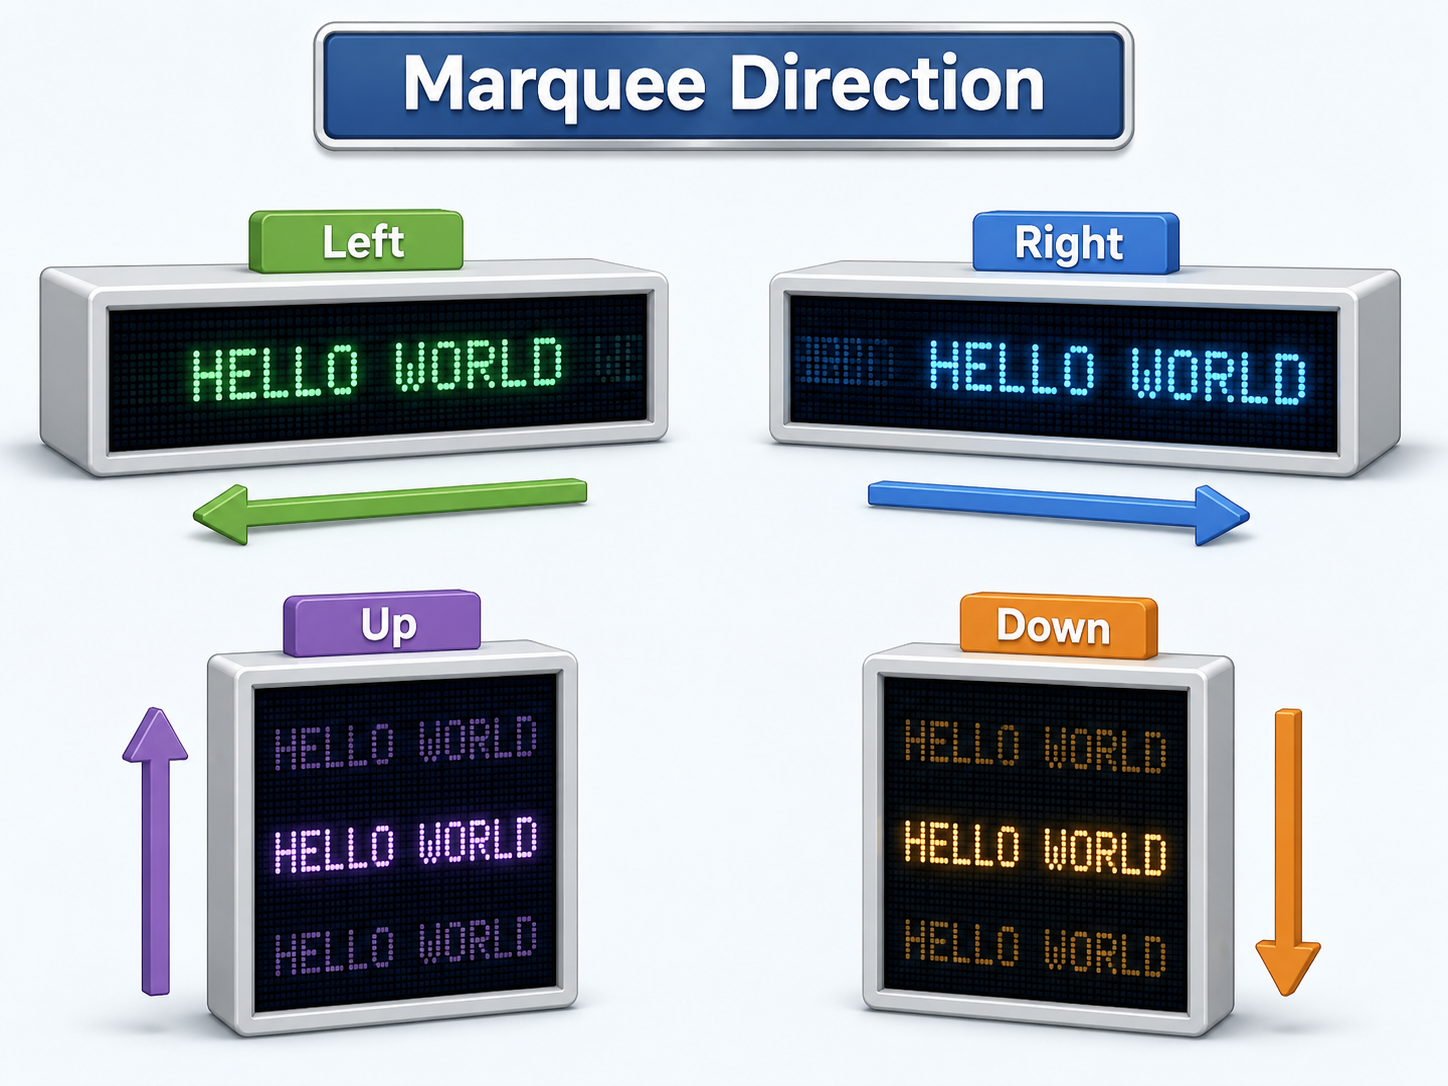
\includegraphics[width=\linewidth,height=.24\textheight,keepaspectratio]{chapters/Chapter04/topics/images/3d_marquee_direction.png}
}{
\fbox{\parbox{0.92\linewidth}{\centering\vspace{0.4cm}
\textbf{চিত্র}\\
ফাইল: \texttt{chapters/Chapter04/topics/images/3d\_marquee\_direction.png}
\vspace{0.4cm}}}
}
\captionof{figure}{চলমান লেখার ট্যাগের \texttt{direction} অ্যাট্রিবিউট}
\end{minipage}\hfill
\begin{minipage}[t]{.46\linewidth}\vspace{0pt}\small
\begin{keypointbox}{চিত্র ব্যাখ্যা}
চিত্রে লেখার চলার চারটি দিক দেখানো হয়েছে। \texttt{left} বামে, \texttt{right} ডানে, \texttt{up} উপরে এবং \texttt{down} নিচে চলার নির্দেশ দেয়।
\end{keypointbox}

\begin{keypointbox}{চিত্র দেখে কোড লেখার ধাপ}
\texttt{<marquee>}-এর ভেতরের লেখা বা ছবি চলমান থাকে। \texttt{direction} অ্যাট্রিবিউটের মান চলার দিক নির্ধারণ করে।
\end{keypointbox}
\end{minipage}\par


\begin{examplebox}{বিশেষভাবে দেখানো HTML কোড}
\par\noindent\begin{minipage}{\linewidth}
\begin{verbatim}
<marquee direction="left">Welcome to HSC ICT</marquee>
<marquee direction="right">HTML Marquee Example</marquee>
<marquee direction="up" height="80">Move Up</marquee>
<marquee direction="down" height="80">Move Down</marquee>
\end{verbatim}
\end{minipage}\par
\end{examplebox}

\begin{mistakebox}{আধুনিক সতর্কতা}
\texttt{<marquee>} বর্তমান HTML-এ পুরোনো ও নতুন কোডে ব্যবহারযোগ্য নয় এমন বৈশিষ্ট্য। পরীক্ষার উদাহরণ বোঝার জন্য এটি জানা দরকার। নতুন ওয়েবসাইটে চলমান দৃশ্যের জন্য CSS অ্যানিমেশন ব্যবহার করা হয়।
\end{mistakebox}

\subsection{লেখা বিন্যাসের ট্যাগ ও কাজ}

\begin{center}
\footnotesize
\begin{tabular}{|p{0.17\textwidth}|p{0.30\textwidth}|p{0.37\textwidth}|}
\hline
\textbf{ট্যাগ} & \textbf{কাজ} & \textbf{উদাহরণ} \\
\hline
\texttt{<h1>--<h6>} & শিরোনাম তৈরি করে & \texttt{<h1>Title</h1>} \\
\hline
\texttt{<p>} & অনুচ্ছেদ তৈরি করে & \texttt{<p>Text</p>} \\
\hline
\texttt{<br>} & নতুন লাইন তৈরি করে & \texttt{Line 1<br>Line 2} \\
\hline
\texttt{<hr>} & অনুভূমিক লাইন তৈরি করে & \texttt{<hr>} \\
\hline
\texttt{<b>} & মোটা অক্ষরের লেখা & \texttt{<b>Bold</b>} \\
\hline
\texttt{<strong>} & গুরুত্বপূর্ণ লেখা & \texttt{<strong>Important</strong>} \\
\hline
\texttt{<i>} & বাঁকা অক্ষরের লেখা & \texttt{<i>Italic</i>} \\
\hline
\texttt{<em>} & জোর দেওয়া লেখা & \texttt{<em>Emphasis</em>} \\
\hline
\texttt{<u>} & নিচে রেখাযুক্ত লেখা & \texttt{<u>Underline</u>} \\
\hline
\texttt{<ins>} & যোগ করা লেখা & \texttt{<ins>New</ins>} \\
\hline
\texttt{<del>} & বাদ দেওয়া লেখা & \texttt{<del>Old</del>} \\
\hline
\texttt{<s>} & মাঝে রেখাযুক্ত & \texttt{<s>Old</s>} \\
\hline
\texttt{<strike>} & মাঝে রেখাযুক্ত পুরোনো ট্যাগ & \texttt{<strike>Old</strike>} \\
\hline
\texttt{<small>} & ছোট লেখা & \texttt{<small>Small</small>} \\
\hline
\texttt{<big>} & বড় লেখা & \texttt{<big>Big</big>} \\
\hline
\texttt{<sub>} & নিচের সূচক & \texttt{H<sub>2</sub>O} \\
\hline
\texttt{<sup>} & উপরের সূচক & \texttt{a<sup>2</sup>} \\
\hline
\texttt{<pre>} & উৎসের বিন্যাস অক্ষুণ্ণ রাখা লেখা & \texttt{<pre>Text</pre>} \\
\hline
\texttt{<font>} & অক্ষরের আকার, রং ও ফন্টের ধরন & \texttt{<font color="red">Text</font>} \\
\hline
\end{tabular}
\normalsize
\end{center}

% Original applied explanation; see Chapter04/SOURCES.md.
\subsubsection{নোটিশের গুরুত্ব ও দেখতে মোটা লেখার পার্থক্য}
\begin{flushleft}\small
\begin{tabularx}{\linewidth}{|p{26mm}|X|X|}\hline
\textbf{বিবেচনা} & \textbf{\texttt{strong}} & \textbf{\texttt{b}}\\\hline
অর্থ & বিষয়বস্তুর বিশেষ গুরুত্ব গঠনে প্রকাশ করে & সাধারণভাবে দৃষ্টি আকর্ষণের অংশ চিহ্নিত করে\\\hline
দেখতে কেমন & মোটা দেখা যেতে পারে & প্রায় একইভাবে মোটা দেখা যেতে পারে; অর্থ এক নয়\\\hline
\end{tabularx}
\end{flushleft}
\textbf{উদাহরণ:} ভর্তি-নোটিশে \textbf{আবেদনের শেষ দিন} বিশেষ গুরুত্বপূর্ণ। \texttt{strong} দিয়ে সেই গুরুত্ব গঠনে প্রকাশ করা যায়।

নতুন বিষয় শুরু করতে শিরোনাম এবং বিস্তারিত লিখতে অনুচ্ছেদ ব্যবহার করবে। ফাঁকা জায়গা বানাতে বারবার \texttt{br} ব্যবহার করলে ছোট পর্দায় বিন্যাস অনিয়মিত হতে পারে। আলাদা অনুচ্ছেদে \texttt{p}, আর চিঠির ঠিকানার মতো একই অংশে প্রয়োজনীয় লাইনবিরতিতে \texttt{br} বেছে নেবে।


\subsection{পূর্ণাঙ্গ উদাহরণ}

\Needspace{6\baselineskip}
\par\noindent{\color{chFourTeal}\bfseries\small কোড: বাম কলাম শেষে ডান কলাম পড়বে}\par
\begin{multicols}{2}
\begin{verbatim}
<body bgcolor="#F5F5F5">

  <h1 align="center">HSC ICT Chapter 4</h1>
  <hr>

  <p>This is a normal paragraph.</p>
  <p><b>This is bold text.</b></p>
  <p><strong>This is important text.</strong></p>
  <p><i>This is italic text.</i></p>
  <p><em>This text is emphasized.</em></p>
  <p><u>This is underline text.</u></p>
  <p><small>This is small text.</small></p>
  <p><big>This is big text.</big></p>

  <p>Water formula: H<sub>2</sub>O</p>
  <p>Math formula: a<sup>2</sup> + b<sup>2</sup></p>

  <p><del>Old Notice</del> <ins>New Notice</ins></p>
  <p><s>Cancelled class</s></p>
  <p><strike>Old HTML tag</strike></p>

  <font size="5" color="blue" face="Arial">
    This text uses font tag.
  </font>

  <pre>
Name      Roll
Sakib     01
Asraful   02
  </pre>

</body>
\end{verbatim}
\end{multicols}


\begin{examplebox}{ফল কী হবে?}
ব্রাউজারে কেন্দ্রে সাজানো শিরোনাম, অনুভূমিক লাইন, মোটা অক্ষরের/বাঁকা অক্ষরের/নিচে রেখাযুক্ত লেখা, H\textsubscript{2}O নিচের সূচক, a\textsuperscript{2}+b\textsuperscript{2} উপরের সূচক, বাদ দেওয়া/যোগ করা লেখা, নীল Arial ফন্ট লেখা এবং আগের বিন্যাসে রাখা সারণির মতো লেখা দেখা যাবে।
\end{examplebox}

\begin{mistakebox}{সাধারণ ভুল}
\par\noindent
\begin{minipage}[t]{.48\linewidth}\vspace{0pt}
\begin{itemize}
\item \texttt{<br>} ট্যাগকে কন্টেইনার ট্যাগ মনে করা।
\item \texttt{<title>} আর \texttt{<h1>} একই মনে করা।
\item \texttt{<b>} ও \texttt{<strong>} ট্যাগের অর্থের পার্থক্য না বোঝা।
\item \texttt{<i>} ও \texttt{<em>} ট্যাগের অর্থগত পার্থক্য না বোঝা।
\end{itemize}
\end{minipage}\hfill
\begin{minipage}[t]{.48\linewidth}\vspace{0pt}
\begin{itemize}
\item \texttt{<sub>} আর \texttt{<sup>} উল্টো করে ফেলা।
\item \texttt{<font>} ট্যাগ আধুনিক HTML-এ বর্তমান মানে ব্যবহারযোগ্য নয় - এই বাড়তি তথ্য না দেওয়া।
\item বাংলা লেখা ঠিক দেখাতে \texttt{UTF-8} না দেওয়া।
\item ট্যাগ ঠিকভাবে বন্ধ না করা।
\end{itemize}
\end{minipage}\par

\end{mistakebox}


\begin{keypointbox}{শিরোনামের স্তর ঠিক রাখবে}
কলেজের পেজের মূল বিষয় \texttt{h1}, তার বিভাগ \texttt{h2} এবং সেই বিভাগের উপবিষয় \texttt{h3} হতে পারে। শুধু ছোট অক্ষর চাই বলে \texttt{h1} থেকে সরাসরি \texttt{h6}-এ যাওয়া ঠিক নয়। যৌক্তিক শিরোনাম স্ক্রিন রিডার ব্যবহারকারীকে পেজের অংশ বুঝতে সাহায্য করে; অক্ষরের দৃশ্যমান মাপ CSS-এ ঠিক করবে।
\end{keypointbox}


\subsection{সংক্ষিপ্ত অনুশীলন}

% Each question keeps its answer beneath it in the same column.
\begin{multicols}{2}
\noindent\begin{minipage}[t]{\linewidth}\vspace{0pt}
\chFourReviewQuestion{শিরোনাম ট্যাগ কয়টি?}
\end{minipage}\par\smallskip
\noindent\begin{minipage}[t]{\linewidth}\vspace{0pt}
\chFourReviewQuestion{অনুচ্ছেদ লেখার ট্যাগ কোনটি?}
\end{minipage}\par\smallskip
\noindent\begin{minipage}[t]{\linewidth}\vspace{0pt}
\chFourReviewQuestion{লাইন বিরতি করার ট্যাগ কোনটি?}
\end{minipage}\par\smallskip
\noindent\begin{minipage}[t]{\linewidth}\vspace{0pt}
\chFourReviewQuestion{অনুভূমিক লাইন তৈরির ট্যাগ কোনটি?}
\end{minipage}\par\smallskip
\noindent\begin{minipage}[t]{\linewidth}\vspace{0pt}
\chFourReviewQuestion{লেখা মোটা অক্ষরের করতে কোন ট্যাগ ব্যবহার হয়?}
\end{minipage}\par\smallskip
\noindent\begin{minipage}[t]{\linewidth}\vspace{0pt}
\chFourReviewQuestion{লেখা বাঁকা অক্ষরের করতে কোন ট্যাগ ব্যবহার হয়?}
\end{minipage}\par\smallskip
\noindent\begin{minipage}[t]{\linewidth}\vspace{0pt}
\chFourReviewQuestion{H\textsubscript{2}O লেখার জন্য কোন ট্যাগ ব্যবহার হবে?}
\end{minipage}\par\smallskip
\noindent\begin{minipage}[t]{\linewidth}\vspace{0pt}
\chFourReviewQuestion{a\textsuperscript{2} লেখার জন্য কোন ট্যাগ ব্যবহার হবে?}
\end{minipage}\par\smallskip
\noindent\begin{minipage}[t]{\linewidth}\vspace{0pt}
\chFourReviewQuestion{\texttt{<font>} ট্যাগের অ্যাট্রিবিউট কী কী?}
\end{minipage}\par\smallskip
\end{multicols}

\Needspace{10\baselineskip}
\subsection{পরীক্ষাভিত্তিক বহুনির্বাচনি প্রশ্ন}

\begin{multicols}{2}
\begin{enumerate}[leftmargin=*,itemsep=5pt]
\item \begin{minipage}[t]{\linewidth}\vspace{0pt}
ব্রাউজারের স্বাভাবিক রীতিতে সবচেয়ে বড় শিরোনাম কোনটি?
\par ক) \texttt{<h6>}
\par খ) \texttt{<h3>}
\par গ) \texttt{<h1>}
\par ঘ) \texttt{<head>}
\end{minipage}

\item \begin{minipage}[t]{\linewidth}\vspace{0pt}
অনুচ্ছেদ ট্যাগ কোনটি?
\par ক) \texttt{<para>}
\par খ) \texttt{<p>}
\par গ) \texttt{<br>}
\par ঘ) \texttt{<hr>}
\end{minipage}

\item \begin{minipage}[t]{\linewidth}\vspace{0pt}
নতুন লাইন তৈরি করতে কোন ট্যাগ ব্যবহৃত হয়?
\par ক) \texttt{<br>}
\par খ) \texttt{<b>}
\par গ) \texttt{<i>}
\par ঘ) \texttt{<u>}
\end{minipage}

\item \begin{minipage}[t]{\linewidth}\vspace{0pt}
H\textsubscript{2}O লেখার জন্য কোন ট্যাগ দরকার?
\par ক) \texttt{<sup>}
\par খ) \texttt{<sub>}
\par গ) \texttt{<small>}
\par ঘ) \texttt{<big>}
\end{minipage}

\item \begin{minipage}[t]{\linewidth}\vspace{0pt}
a\textsuperscript{2} লেখার জন্য কোন ট্যাগ দরকার?
\par ক) \texttt{<sub>}
\par খ) \texttt{<sup>}
\par গ) \texttt{<del>}
\par ঘ) \texttt{<ins>}
\end{minipage}

\item \begin{minipage}[t]{\linewidth}\vspace{0pt}
\texttt{<font>} ট্যাগের অ্যাট্রিবিউট কোনগুলো?
\par ক) \texttt{size}, \texttt{color}, \texttt{face}
\par খ) \texttt{src}, \texttt{alt}, \texttt{width}
\par গ) \texttt{href}, \texttt{target}, \texttt{title}
\par ঘ) \texttt{rowspan}, \texttt{colspan}, \texttt{border}
\end{minipage}
\end{enumerate}
\end{multicols}

\chFourMCQAnswer{১-গ, ২-খ, ৩-ক, ৪-খ, ৫-খ, ৬-ক}
